%!TEX program = xelatex
% \documentclass[dvips,11pt]{beamer}
\documentclass{beamer}
    \usepackage{xeCJK,subfigure}
    % \setCJKmainfont{Adobe Song Std}
    % \setCJKmainfont{楷体}
    \usetheme{Warsaw}
    \usecolortheme{rose}
    % \title{你好!beamer}
    \date{2017 11}
\begin{document}

% \begin{frame}
%     \titlepage
% \end{frame}

\begin{frame}
    \frametitle{目录}
    \tableofcontents
    % \tableofcontents[pausesections]   
\end{frame}

% \section{性能比较}
% \begin{frame}
%     \frametitle{准确率与耗时}
%     \begin{itemize}
%         \item R-CNN \\
%         在20类的 PASCAL VOC 2010上mAP达到53.7\%,而以往的DPM在这个数据集上是33.4\%,在200类数据集ILSVRC 2013上的目标检测数据集上,mAP是31.4\%
%         耗时:在GPU上一张图像生成proposal box和提取特征耗时13s,cpu上耗时53s
%     \end{itemize}
% \end{frame}

% rcnn
\section{R-CNN 2013}

\begin{frame}
    \frametitle{数据流程图}
    \framesubtitle{2013 Rich feature hierarchies for accurate object detection and semantic segmentation}
    \begin{figure}
        \centering
        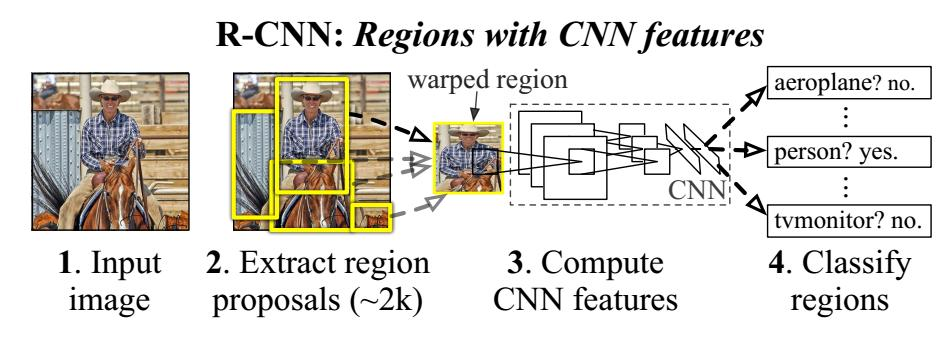
\includegraphics[height=4cm]{graphic/rcnnflow.eps}
    \end{figure}
    输入:图像及selective search算法提出的2000个proposal box。  \\
    输出:proposal box包含的目标类别,及修正后的位置坐标。  \\
\end{frame}

\begin{frame}
    \frametitle{proposal box的形状变换}
    % \framesubtitle{proposal box的变换}
    \begin{figure}
        \centering
        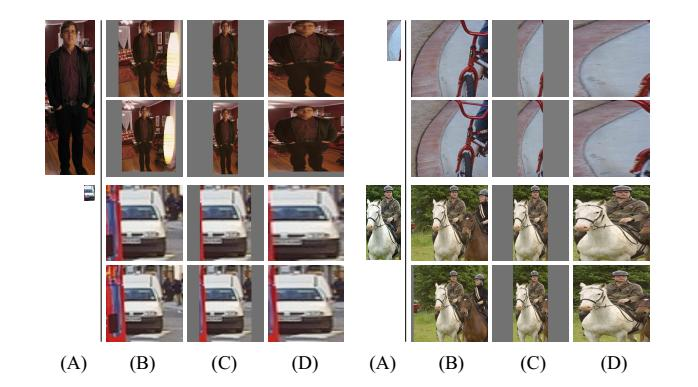
\includegraphics[height=5cm]{graphic/rcnnwarp.eps}
    \end{figure}
    \scriptsize{A是原图的proposal box,B是proposal box的最小外接正方形,短边使用原图填充,然后放大到$227\times 227$,C与B的相同,只是填充短边时使用图像均值,D是直接 warp,即直接进行放大。每列图像,上一行是直接对proposal box处理,即 context padding = 0,下一行的 context padding = 16。实验表明使用D方法中的 warp with context padding = 16时,效果最好,提高3-5 mAP\%}
\end{frame}

\begin{frame}
    \frametitle{特征提取网络}
    \begin{figure}
        \centering
        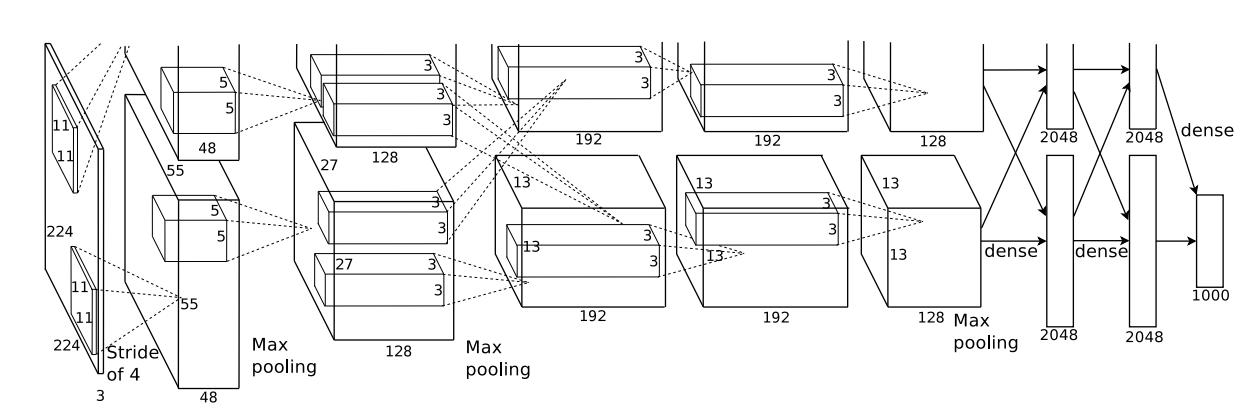
\includegraphics[height=3.7cm]{graphic/alexnet.eps}
    \end{figure}
    采用了和Alexnet一样的结构,5层卷积,3层全连接的分类网路。在做特征提取时,只计算到第二层全连接输出4096维特征向量。
\end{frame}

\begin{frame}
    \frametitle{proposal box的分类}
    这里使用category-specific linear SVM对上一步中proposal box中提取的$4096$维特征向量进行分类。 \\
    \vspace{10pt}
    测试时,一张图像提出$2000$个proposal box,对应的特征向量写成一个矩阵就是$2000\times 4096$维, 乘以 SVM系数矩阵$4096\times N$ (N指目标类别数目)得到每一个proposal box的分数。%之后使用单独为每一类的输出做非极大值抑制,就是去掉那些与有更高分数的proposal box的IOU超过一个阈值的框。
\end{frame}

\begin{frame}
    \frametitle{class-specific bounding box regressor}
    proposal box的参数表示: $P^i=(P_x^i,p_y^i,p_w^i,p_h^i)$ \\
    ground truth box的参数表示: $G=(G_x^i,G_y^i,G_w^i,G_h^i)$ \\
    回归的目标: \\
    $$\begin{aligned} 
        t_x &= (G_x-P_x)/P_w \\
        t_y &= (G_y-P_y)/P_h \\
        t_w &= \log(G_w/P_w)=\log(G_w)-\log(P_w) \\
        t_h &= \log(G_h/P_h)=\log(G_h)-\log(P_h)
    \end{aligned}$$
    \vspace{6pt}
    回归使用的是线性模型,损失函数是均方误差加上$L_2$正则项: 
    $$loss=\sum_i^N (t_{\star}^i-\hat w_{\star}^T \phi_5(P^i))^2+\lambda\|\hat w_{\star}\|^2$$
    \scriptsize{其中,$\phi_5(P^i)$表示CNN的pool 5层在proposal box内提取的特征,$w_{\star}$表示回归要学习的参数。}
\end{frame}

\begin{frame}
    \frametitle{IOU}
    Intersection Over Union:两个框重叠度的计算 \\
    \begin{figure}
        \centering
        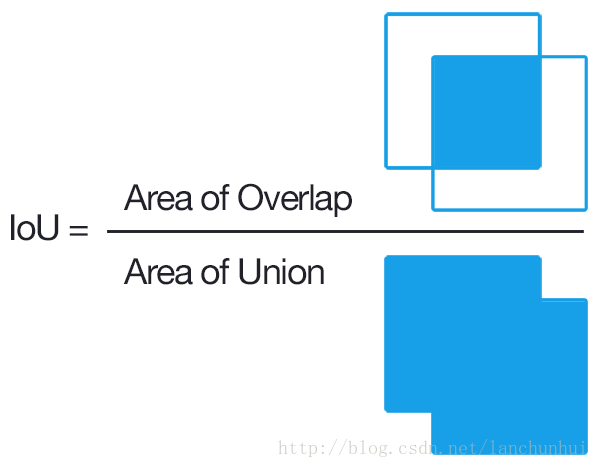
\includegraphics[height=4cm]{graphic/iou.eps}
    \end{figure}
\end{frame}

\begin{frame}
    \frametitle{训练}
    \begin{itemize}
        \item CNN的训练 \\
        先在ILSVRC2012图像分类数据集上进行预训练,之后在目标检测数据集VOC与ILSVRC203上进行微调,微调时把proposal box中所有与ground-truth box的IOU大于0.5的框看做正样本,其余的proposal box都是负样本。训练时,batch-size为128,其中32个为正样本,96个背景样本。        
        \item SVM的训练样本 \\
        正样本只有ground-truth box提出的特征,负样本是propoal box中与ground-truth box的IOU小于0.3的。
        \item bounding-box regressor的训练样本   \\
        对于每一个proposal box,计算它与所有的ground-truth box的IOU,然后选出IOU最大的那一个,如果此IOU值大于$0.6$,那么这个proposal box就配对成功,看做一个训练样本,配对不成功的proposal box被舍弃。
    \end{itemize}
\end{frame}

% fast rcnn
\section{Fast R-CNN 2015}

\begin{frame}
    \frametitle{数据流程图}
    \framesubtitle{2015 Fast R-CNN}
    \begin{figure}
        \centering
        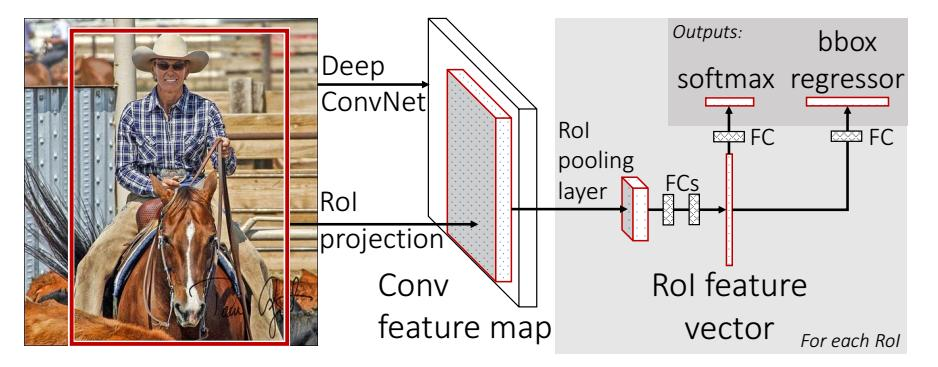
\includegraphics[height=4.3cm]{graphic/fastrcnnflow.eps}
    \end{figure}
    输入:图像及selective search算法提出的2000个proposal box。  \\
    输出:proposal box包含的目标类别,及修正后的位置坐标。  \\
\end{frame}

% \begin{frame}
%     \frametitle{ROI pooling}
%     ROI:region of interest,就是特征图上的一个矩形,对应到原图的proposal box, \\
%     \begin{figure}
%         \centering
%         \includegraphics[width=0.35\textwidth]{graphic/roipooling0.jpg}%
%         \includegraphics[width=0.35\textwidth]{graphic/roipooling1.jpg}%
%         \includegraphics[width=0.35\textwidth]{graphic/roipooling2.jpg}
%     \end{figure}
%     卷积网络输出为$8\times 8$的特征图,这里的一个左上角坐标为$(0,3)$,右下角坐标为$(6,7)$,长宽分别为$7,5$的roi一个Roi对应$2\times 2$的固定长度的特征向量输出。
% \end{frame}

% \begin{frame}
%     \frametitle{ROI pooling}
%     \begin{figure}
%         \centering
%         \includegraphics[width=0.5\textwidth]{graphic/roipooling3.jpg}%
%         \includegraphics[width=0.5\textwidth]{graphic/roipooling4.jpg}%
%     \end{figure}
%     Roi pooling使不同大小,不同长宽比的proposal box都能提取到固定长度的特征向量。
% \end{frame}
\begin{frame}
    \frametitle{ROI pooling}
    \begin{figure}
        \centering
        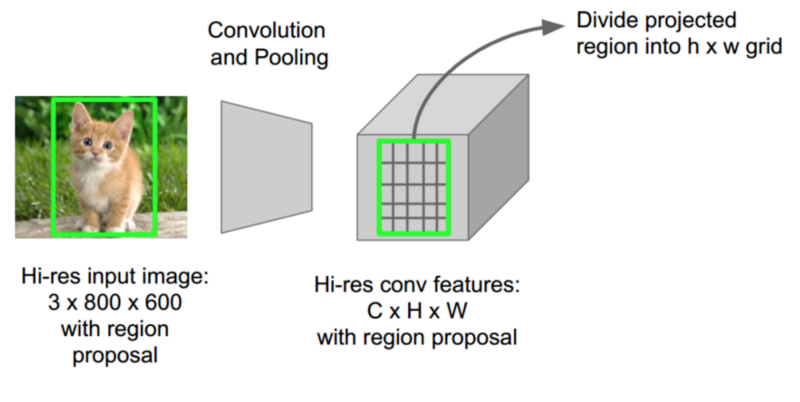
\includegraphics[width=1.0\textwidth]{graphic/roipooling6.png}
    \end{figure}
    Roi pooling使不同大小,不同长宽比的proposal box都能提取到固定长度的特征向量。
\end{frame}


\begin{frame}
    \frametitle{Multi-task loss}
    分类器与坐标回归的损失函数:
    $$L(p,u,t^u,v)=L_{cls}(p,u) + \lambda [u\geqslant 1]L_{loc}(t^u,v)$$
    其中,p为预测的分类概率,u真实分类的label,$t^u$为预测的坐标偏差,因为坐标回归针对每一类都有一个回归器,所以它是$u$的函数,v为真实的坐标偏差label,$[u\geqslant 1]$艾佛森括号,表示$u\geqslant 1$时,输出为1,否则为0。
\end{frame}

\begin{frame}
    \frametitle{Multi-task loss}
    分类器与坐标回归的损失函数:
    $$L(p,u,t^u,v)=L_{cls}(p,u) + \lambda [u\geqslant 1]L_{loc}(t^u,v)$$
    分类损失:
    $$L_{cls}=-\log p_u$$
    坐标回归损失:
    $$L_{loc}(t^u,v)=\sum_{i\in \{x,y,w,h\}}smooth_{L1}(t^u_i-v_i)$$
    与R-CNN不同,这里使用了$Smooth_{L1}$损失:
    $$smooth_{L1}(x) = \begin{cases} 
        0.5x^2 &\text{if }|x| < 1 \\
        |x| - 0.5 &\text{otherwise}\end{cases}  \rightarrow \text{求导}
    \begin{cases} x \\ \pm 1 \end{cases}$$
\end{frame}

% \section{Faster R-CNN}
% \begin{frame}
%     \frametitle{数据流程图}
%     \framesubtitle{2015 faster rcnn: towards real-time object detection with region proposal networks}
%     \begin{minipage}[c]{0.6\linewidth}
%         \centering
%         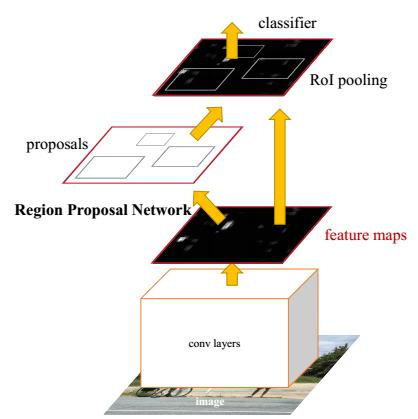
\includegraphics[width=1.0\textwidth]{graphic/fastercnnflow.jpg}
%     \end{minipage}%
%     \begin{minipage}[c]{0.45\linewidth}
%         Faster R-CNN相当于RPN与Fast R-CNN的结合体,图中左边是RPN,右边是Fast R-CNN。
%     \end{minipage}
% \end{frame}

% \begin{frame}
%     \frametitle{RPN中的多尺度}
%     \begin{figure}
%         \centering
%         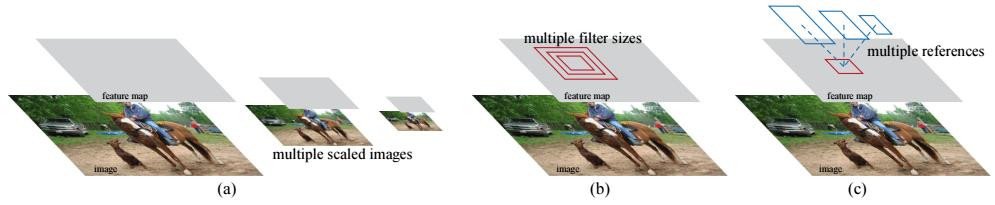
\includegraphics[width=1.0\textwidth]{graphic/fastermultisize.jpg}
%     \end{figure}
%     $(a)$图通过图像金字塔构造多尺度,$(b)$图是通过构造滤波器的金字塔构造多尺度,$(c)$图是使用一个尺度的滤波器,得到一个尺度的特征图,然后在特征图上选不同大小的框来构造多尺度。
% \end{frame}

% \begin{frame}
%     \frametitle{RPN网络的输出}
%     \begin{figure}
%         \centering
%         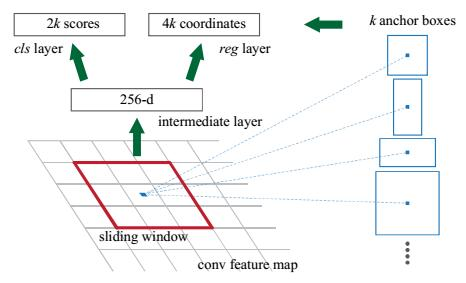
\includegraphics[width=0.8\textwidth]{graphic/rpnout.jpg}
%     \end{figure}
%     以$3\times 3$大小的滑动窗口在特征图上滑动。
% \end{frame}

% \begin{frame}
%     \frametitle{RPN网络的损失函数}
%     $$L(\{p_i\}, \{t_i\})=\frac{1}{N_{cls}}\sum_i L_{cls}(p_i,p_i^*)+\lambda \frac{1}{N_{reg}}\sum_i p_i^* L_{reg}(t_i,t_i^*)$$ \\
%     其中,$p_i$表示预测的一个anchor为目标的概率,$p_i^*$表示一个anchor的label为1或0,
%     $t_i$表示预测的4个参数化的bounding box,$t_i^*$表示一个关于正样本anchor的ground truth box,
%     这里regression loss选用了smooth L1损失,分类层与回归层的输出分别为$\{p_i\}$和$\{t_i\}$,$N_{cls}$表示mini-batch的大小,$N_{reg}$表示anchor的数量(一张图像里的,2400)。
% \end{frame}
% \begin{frame}
%     \frametitle{Faster R-CNN的训练}
%     1,单独训练RPN;\\
%     2,使用步骤中1得到的区域生成方法单独训练Fast R-CNN; \\
%     3, 使用步骤2得到的网络作为初始网络训练RPN;\\
%     4, 再次训练Fast R-CNN, 微调参数。\\
% \end{frame}

\end{document}